\ifspanish

Un videojuego consta de $N$ niveles consecutivos, $0, 1, ..., N-1$. El jugador empieza en el nivel 0. Si un jugador pasa el nivel $i$, entra en el nivel $i+1$, si no, vuelve al nivel 0. Se sabe que todas las fases tienen la misma dificultad, por lo que si jugador está en el nivel $i$, alcanza el nivel $i+1$ con probabilidad $q$, y regresa a 0 con probabilidad $1-q$.

Cuando el jugador alcanza la etapa $N-1$, obtiene una medalla, vuelve al nivel 0 y el juego continúa.

Sea $X_k$ el proceso estocástico que representa la secuencia de niveles durante un juego, tal que $X_k=i$ significa que el jugador estaba en el nivel $i$ en el momento $k$. El juego comienza en $X_0=0$.
\begin{parts}
\part Formule el problema como un proceso de Markov estacionario y dibuje el gráfico de transición para $N = 6$.
\part Asumiendo $N \ge 2$, calcule $P\{X_2=1\}$.
\part Suponiendo $N \ge 2$, determine la probabilidad de obtener una medalla exactamente en el tiempo $k$, es decir $P\{X_k=N-1\}$, para $k=0,1, \ldots, N$.
\part Para $N=2$, determine la distribución estacionaria.
\part Para $N=\infty$, determine la distribución estacionaria

\end{parts}

\begin{solution}
\begin{parts}
\part El grafo de transición se muestra en la figura para $q=0.1$.

{\centering
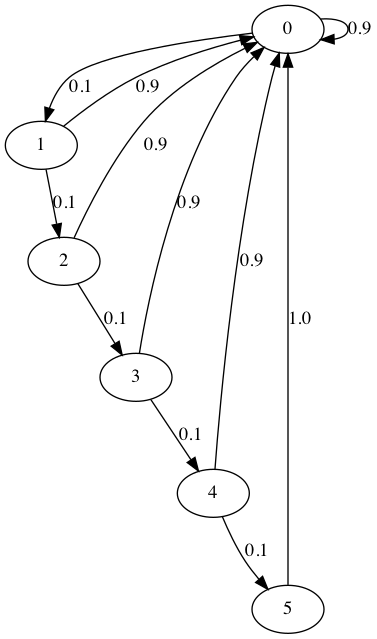
\includegraphics[scale=0.3]{db/figs/SPES_202106_markov_chain.png}}

\part 
\begin{align*}
P\{X_2=1\} = q P\{X_1=0\} = q (1-q) P\{X_0=0\} = q (1-q) 
\end{align*}

\part La probabilidad de obtener una medalla en el momento $k$ es $Q_k=P\{X_k=N-1\}$. Daddo que se requieren al menos $N-1$ pasos para alcanzar el nivel $N-1$, resulta
\begin{align*}
Q_k = 0,     \qquad \text{ for } k=0, \ldots, N-2
\end{align*}

Alcanzar el nivel $N-1$ en el momento $k=N-1$ is posible solamente si el jugador no falla en ninguna ocasión, de modo que
\begin{align*}
Q_{N-1} = q^{N-1}
\end{align*}

Alcanzar el nivel $N-1$ en $k=N$ es posible solamente si el jugador falla en el instante $0$ únicamente, de modo que
\begin{align*}
Q_{N} = (1-q) q^{N-1}
\end{align*}

\part Dado que
\begin{align*}
\pi_1 = q \pi_0
\end{align*}
y $\pi_0 + \pi_1 = 1$, resulta
\begin{align*}
\pi_1 = \frac{q}{1+q}
\end{align*}

\part Para $i>0$, se tiene que
\begin{align*}
\pi_i = q \pi_{i-1} = q^2 \pi_{i-2} = \ldots = q^i \pi_0
\end{align*}
y, para $i=0$,
\begin{align*}
\pi_0 = \sum_{i=0}^\infty (1-q) \pi_i 
       = (1-q) \sum_{i=0}^\infty \pi_i 
       = 1-q
\end{align*}
de modo que
\begin{align*}
\pi_i = (1-q) q^i
\end{align*}

\end{parts}
\end{solution}

\else

A video game consists of $N$ consecutive levels, $0, 1, ..., N-1$. The player starts at level 0. If a player passes level $i$, she enters level $i+1$, if not, she returns back to level 0. It is known that all phases have the same difficulty, so, if a player is at level $i$, she reaches level $i+1$ with probability $q$, and returns back to 0 with probability $1-q$. 

When the player reaches stage $N-1$, she gets a medal, returns to level 0 and the game continues.

Let $X_k$ be the stochastic process that represents the sequence of levels during a game, such that $X_k=i$ means that the player was at level $i$ at time $k$. The game begins at $X_0=0$.
\begin{parts}
\part Formulate the problem as a stationary Markov process, and draw the transition graph for $N = 6$.
\part Assuming $N \ge 2$, compute $P\{X_2=1\}$.
\part Assuming $N \ge 2$, determine the probability of obtaining a medal exactly at time $k$, that is $P\{X_k=N-1\}$, for $k=0,1, \ldots, N$.
\part For $N=2$, determine the stationary distribution.
\part For $N=\infty$, determine the stationary distribution

\end{parts}

\begin{solution}
\begin{parts}
\part The transition graph is shown in the figure for $q=0.1$.

{\centering
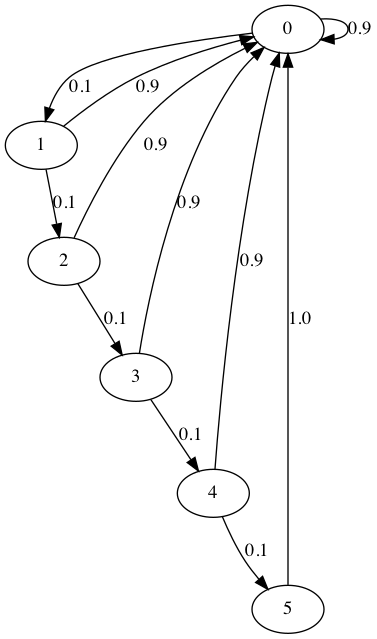
\includegraphics[scale=0.3]{db/figs/SPES_202106_markov_chain.png}}

\part 
\begin{align*}
P\{X_2=1\} = q P\{X_1=0\} = q (1-q) P\{X_0=0\} = q (1-q) 
\end{align*}

\part The probability of obtaining a medal at time $k$ is $Q_k=P\{X_k=N-1\}$. Since at least $N-1$ steps are required to reach level $N-1$, we have
\begin{align*}
Q_k = 0,     \qquad \text{ for } k=0, \ldots, N-2
\end{align*}

Reaching level $N-1$ at time $k=N-1$ is possible only if the player does not fail at any time, so that
\begin{align*}
Q_{N-1} = q^{N-1}
\end{align*}

Reaching level $N-1$ at time $k=N$ is possible only if the player fails at time $0$ only, so that.
\begin{align*}
Q_{N} = (1-q) q^{N-1}
\end{align*}

\part Since
\begin{align*}
\pi_1 = q \pi_0
\end{align*}
and $\pi_0 + \pi_1 = 1$, we have
\begin{align*}
\pi_1 = \frac{q}{1+q}
\end{align*}

\part For $i>0$, we have
\begin{align*}
\pi_i = q \pi_{i-1} = q^2 \pi_{i-2} = \ldots = q^i \pi_0
\end{align*}
and, for $i=0$,
\begin{align*}
\pi_0 = \sum_{i=0}^\infty (1-q) \pi_i 
       = (1-q) \sum_{i=0}^\infty \pi_i 
       = 1-q
\end{align*}
so that
\begin{align*}
\pi_i = (1-q) q^i
\end{align*}

\end{parts}
\end{solution}


\fi